\chapter{Resultados}

\section{Evaluaci�n de Resultados}

Los siguientes resultados fueron evaluaciones de m�todos de proyecci�n usando un parte la herramienta \citep{paulovich2007projection}, haciendo tambi�n uso de conjuntos de datos temporales. Se contrastaron los m�todos de proyecci�n con medicines de distancia o similitud comunes como son la distancia euclidina y especificas para series temporales como son \textit{Dynamic time warping}.

\subsection{Synthetic Control Chart}
Esta conjunto de datos temporales fueron extra�dos de \citep{UCRArchive}, y consta de 6 clases: \textit{Normal, Cyclic, Increasing trend, Decreasing trend, Upward shift y Downward shift} con 600 muestras de 60 dimensiones cada series de tiempo.
Las figuras \ref{fig:sc_idmap_euclidiana}, \ref{fig:sc_idmap_dtw} muestran las propuestas hechas en \citep{alencar2007mineraccao}, donde se hace uso del m�todo de proyecci�n IDMAP con datos temporales usando distancia euclidiana y el \textit{dynamic time warping} respectivamente.

 En las figuras \ref{fig:sc_nj_euclidiana}, \ref{fig:sc_nj_dtw}, se observa el comportamiento del m�todo de proyecci�n \textit{Neighbours joining} tanto con distancia euclidiana como \textit{dynamic time warping}.

% \ref{fig:sc_idmap_euclidiana}, \ref{fig:sc_idmap_dtw}, \ref{fig:sc_nj_euclidiana}, \ref{fig:sc_nj_dtw}.

\begin{figure}[!tbp]
	\centering
	\begin{minipage}[b]{0.52\textwidth}
		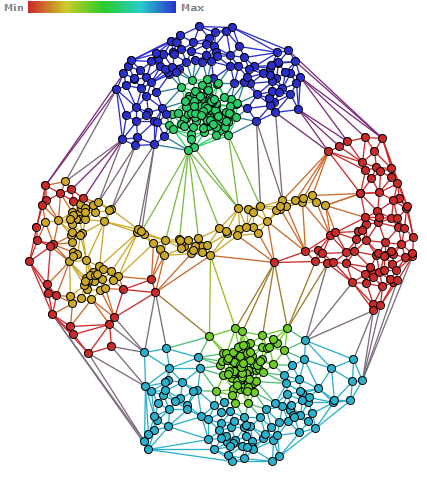
\includegraphics[width=\textwidth]{imagenes/resultados/sc_idmap_euclidiana.png}
		\caption{Proyecci�n IDMAP con distancia euclidiana}
		\label{fig:sc_idmap_euclidiana}
	\end{minipage}
	\hfill
	\begin{minipage}[b]{0.4\textwidth}
		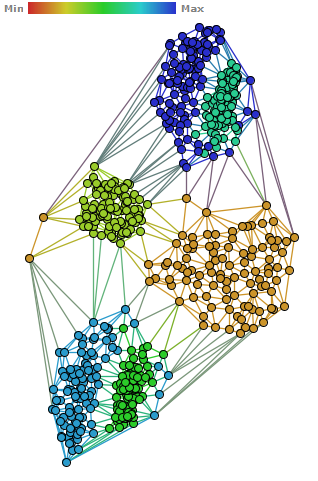
\includegraphics[width=\textwidth]{imagenes/resultados/sc_idmap_dtw.png}
		\caption{Proyecci�n IDMAP con distancia DTW}
		\label{fig:sc_idmap_dtw}
	\end{minipage}
\end{figure}


\begin{figure}[!tbp]
	\centering
	\begin{minipage}[b]{0.55\textwidth}
		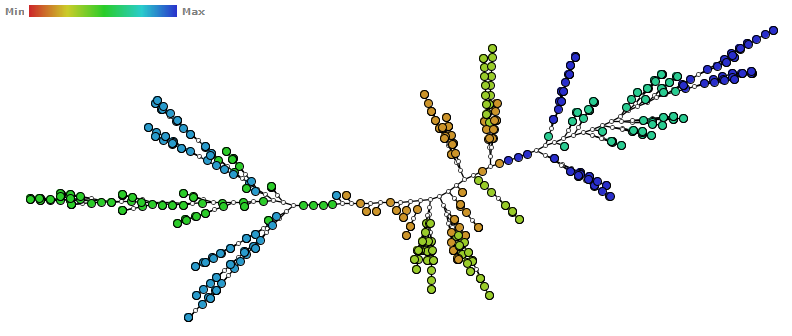
\includegraphics[width=\textwidth]{imagenes/resultados/sc_nj_euclidiana.png}
		\caption{ Proyecci�n NJ con distancia euclidiana}
		\label{fig:sc_nj_euclidiana}
	\end{minipage}
	\hfill
	\begin{minipage}[b]{0.4\textwidth}
		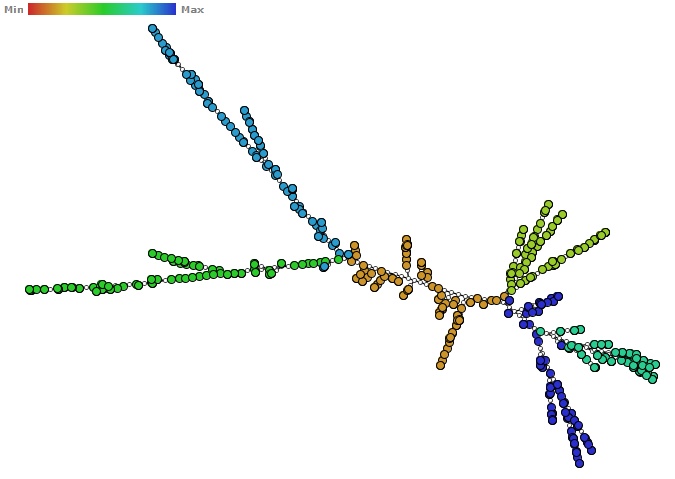
\includegraphics[width=\textwidth]{imagenes/resultados/sc_nj_dtw.png}
		\caption{Proyecci�n NJ con distancia DTW}
		\label{fig:sc_nj_dtw}
	\end{minipage}
\end{figure}


\subsection{Gun Point}
Disponibles tambi�n en \citep{UCRArchive}, contiene 2 clases, con un total de 200 registros y una longitud de series de tiempo de 150. Este conjunto de datos posee como se hab�a mencionado antes posee dos clases las cuales son \textit{Point} y \textit{Gun}, siendo la principal diferencia que en una el personaje apunta con su dedo mientras en el otro grupo con un arma.
Este conjunto es de dif�cil an�lisis pues las dos clases no presentan grandes diferencias. En la figuras \ref{fig:gp_lsp_dtw}, \ref{fig:gp_nj_dtw} se muestran las proyecciones LSP y NJ usando la distancia DTW.

\begin{figure}[!tbp]
	\centering
	\begin{minipage}[b]{0.4\textwidth}
		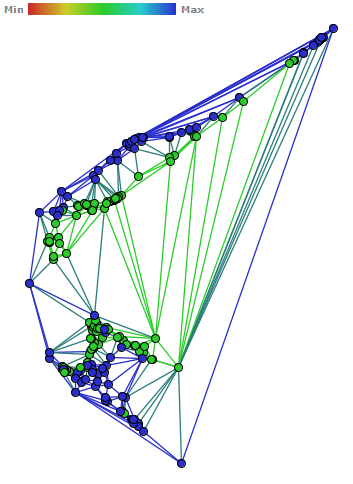
\includegraphics[width=\textwidth]{imagenes/resultados/gp_lsp_dtw.png}
		\caption{Proyecci�n LSP con distancia DTW}
		\label{fig:gp_lsp_dtw}
	\end{minipage}
	\hfill
	\begin{minipage}[b]{0.4\textwidth}
		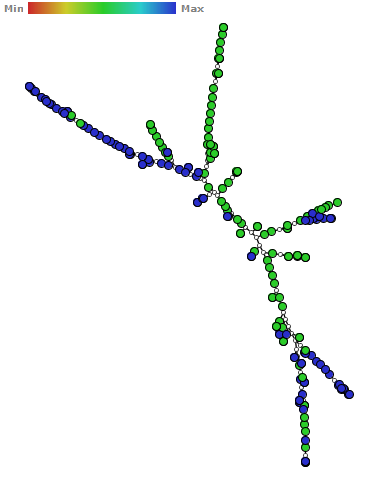
\includegraphics[width=\textwidth]{imagenes/resultados/gp_nj_dtw.png}
		\caption{Proyecci�n NJ con distancia DTW}
		\label{fig:gp_nj_dtw}
	\end{minipage}
\end{figure}


\subsection{Alessandro Vespignani dataset}
Es un conjunto de res�menes de art�culos relacionados que tienen como autor a Alessandro Vespignami entre los a�os 1990 al 2012. Cuenta con informaci�n como a�o de publicaci�n referencias, resumen etc. Este conjunto de datos a sido usado en \citep{alencarvisualizaccao}. La figura \ref{fig:t_lsp} muestra los resultados obtenidos por \citep{alencarvisualizaccao}, mientras en la figura \ref{fig:t_nj} se utilizo esta misma base de datos usando la proyecci�n \textit{Neighbours joining}.
En \ref{fig:t_lsp} los puntos son art�culos cient�ficos, los enlaces son las referencias entre art�culos, y el color esta dado por la fecha de publicaci�n de cada articulo. En la figura \ref{fig:t_nj} se pierde las referencias bibliogr�ficas, pero en su modelo de �rbol permite ver la relaci�n local entre documentos, aun as� el a�o de publicaci�n aun se muestra de manera desordenada.  


\begin{figure}[!tbp]
	\centering
	\begin{minipage}[b]{0.4\textwidth}
		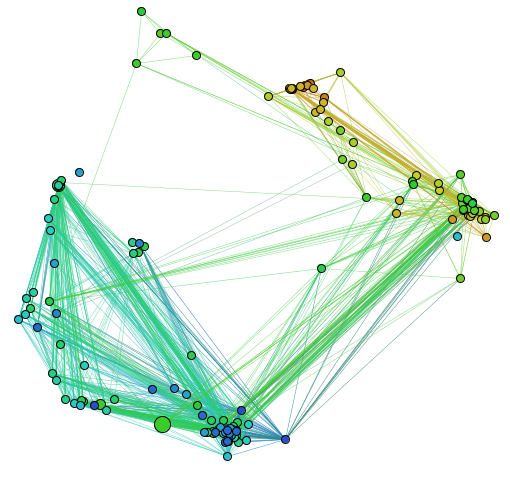
\includegraphics[width=\textwidth]{imagenes/resultados/t_lsp.png}
		\caption{Proyecci�n temporal LSP usando de dataset colecciones de documentos}
		\label{fig:t_lsp}
	\end{minipage}
	\hfill
	\begin{minipage}[b]{0.5\textwidth}
		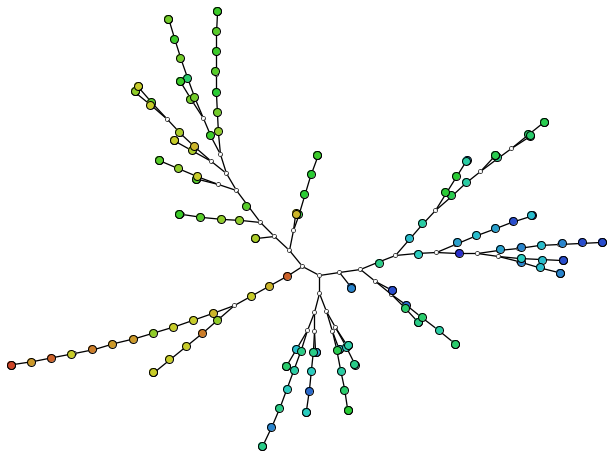
\includegraphics[width=\textwidth]{imagenes/resultados/t_nj.png}
		\caption{Proyecci�n NJ usando de dataset colecciones de documentos}
		\label{fig:t_nj}
	\end{minipage}
\end{figure}
